\section{Solving the Vehicle Routing Problem with Time Windows (VRPTW) Using Ant Colony Optimization (ACO) and Particle Swarm Optimization (PSO)}
The VRPTW was a variant of the Vehicle Routing Problem (VRP), which was crucial in logistics, transportation, and supply chain management. In VRPTW, a fleet of vehicles had to deliver goods to multiple customers. Each customer had a specific time window during which the delivery had to occur. The challenge was to design routes that minimized the total travel distance while ensuring all deliveries met their respective time constraints. This task focused on optimizing the delivery routes for a fleet of vehicles using two nature-inspired optimization algorithms: Ant Colony Optimization (ACO) and Particle Swarm Optimization (PSO). 
\newline
We defined the objective as finding the most efficient routes for a set of vehicles, ensuring that all customers receive their deliveries within specified time windows.
\newline
We implemented both Ant Colony Optimization and Particle Swarm Optimization to solve the Vehicle Routing Problem with Time Windows. We then compared the effectiveness of these algorithms. 
\newline
The primary objective of the VRPTW is to minimize the total distance travelled by all vehicles 
while ensuring that: 
\newline
\newline 1. Each customer is visited exactly once by one vehicle. 
\newline 2. Deliveries occur within the specified time windows. 
\newline 3. The total demand on any route does not exceed the vehicle's capacity. 
\subsection{Data Exploration, and pre processing}
We used Solomon’s VRPTW Benchmark Problems dataset, C101.txt [5].
\newline
The columns in the dataset are:
\newline
CUST NO.: Customer number (ID).
\newline
XCOORD: X coordinate of the customer's location.
\newline
YCOORD: Y coordinate of the customer's location.
\newline
DEMAND: The demand at the customer location.
\newline
READY TIME: The earliest time at which service can begin.
\newline
DUE DATE: The latest time by which the service should be completed.
\newline
SERVICE TIME: The time it takes to complete the service for this customer.
\subsection{Define the VRPTW}
From information above, and given dataset, we can define the VRPTW as follows[15]:
\begin{itemize}
    \item Let \( K \) be the number of vehicles.
    \item Let \( N \) be the number of customers.
    \item The objective is to minimize the total travel distance.
\end{itemize}

The variables involved are:
\begin{itemize}
    \item \( x_{ijk} \): A binary variable indicating if vehicle \( k \) travels directly from customer \( i \) to customer \( j \).
    \item \( t_i \): The arrival time of vehicle \( k \) at customer \( i \).
    \item \( q_i \): The demand of customer \( i \).
\end{itemize}

\subsection{Time Windows}
To calculate the time window, we need the Time Window formula for our problem. For each customer \( i \), the time window is defined as:
\[
\text{Time Window}_i = [\text{READY TIME}_i, \text{DUE DATE}_i]
\]

Where:
\begin{itemize}
    \item \( \text{READY TIME}_i \) is the earliest time at which the service can start for customer \( i \).
    \item \( \text{DUE DATE}_i \) is the latest time by which the service must be completed for customer \( i \).
\end{itemize}

The vehicle must arrive at customer \( i \) within the specified time window.
\begin{figure}[H]
    \centering
    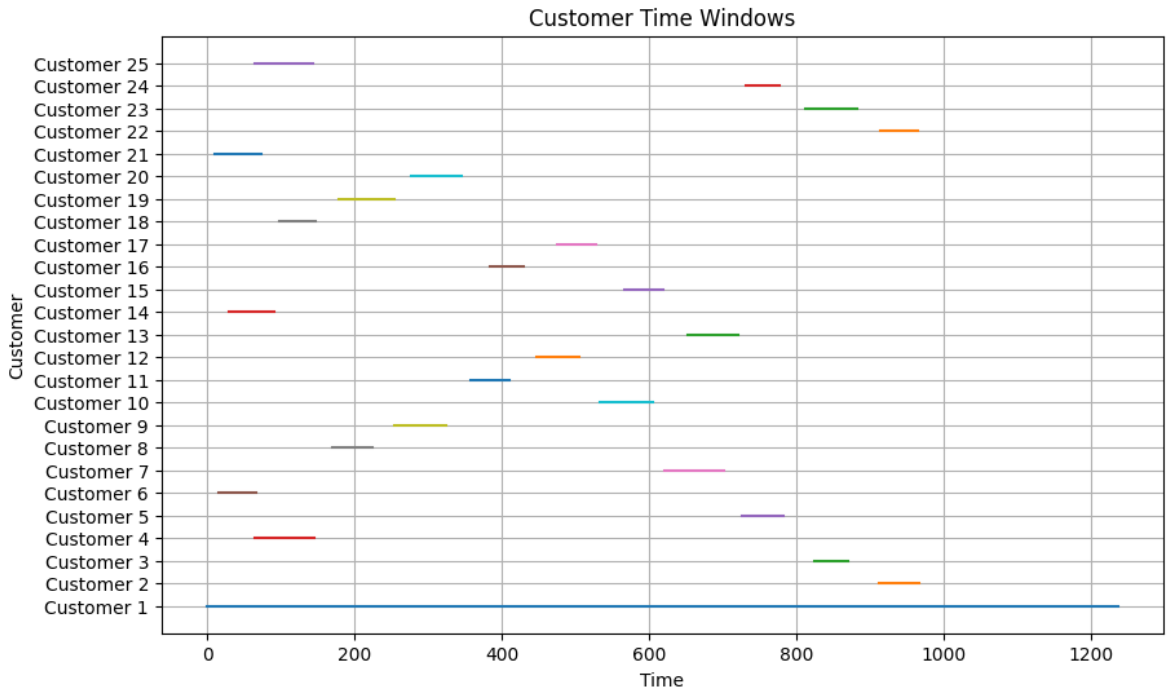
\includegraphics[width=0.8\linewidth]{figures/Customer_Time_Window.PNG}
    \caption{Customer Time Windows}
    \label{fig:Customer Time Windows}
\end{figure}

\subsection{City Coordinate}
In order to calculate city Coordinate, we need to define city Coordinates Formula[17]. 
\newline
City Coordinates Formula:
\newline
For each customer \(i\), the city coordinates are defined as:

\[
\text{City Coordinates}_i = (X_i, Y_i)
\]

Where:
\begin{itemize}
    \item \( X_i \) is the \(x\)-coordinate (longitude or horizontal distance) of the customer's location.
    \item \( Y_i \) is the \(y\)-coordinate (latitude or vertical distance) of the customer's location.
\end{itemize}
\begin{figure}[H]
    \centering
    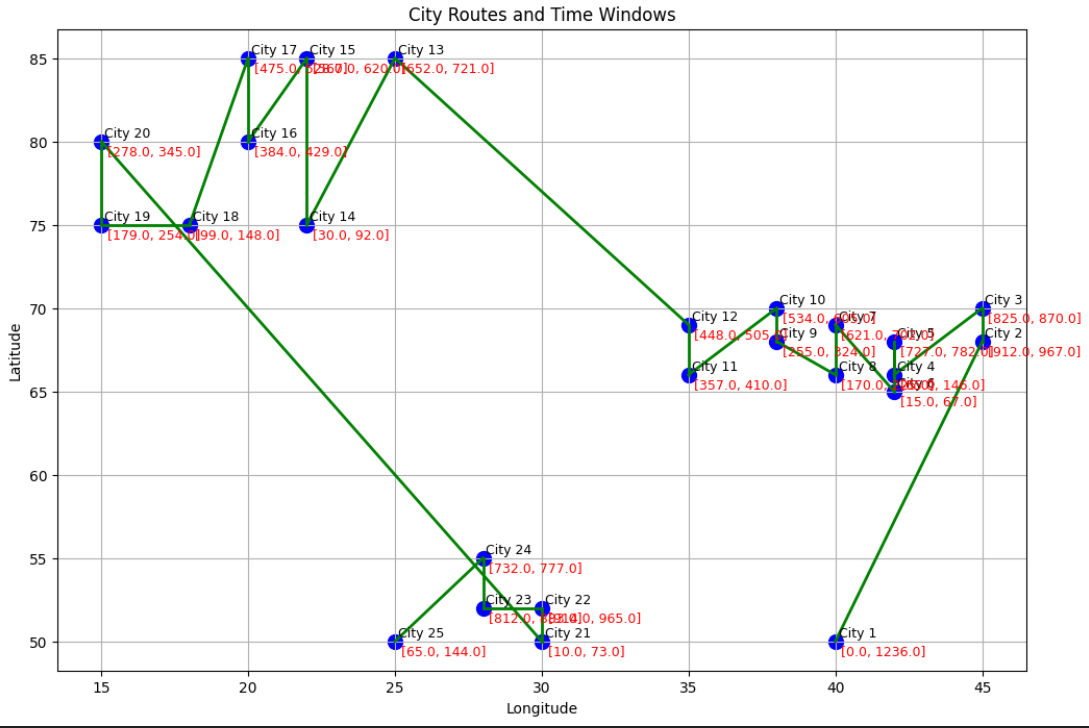
\includegraphics[width=0.8\linewidth]{figures/Citye_Routes_And_Time_Windows.PNG}
    \caption{City Routes And Time Windows}
    \label{fig:City Routes And Time Windows}
\end{figure}
\subsection{Dist Matrix}
To calculate the distance between two customers \(i\) and \(j\) based on their coordinates, we use the Euclidean distance formula[17]:
\newline Distance Formula:
\newline
\[
d_{ij} = \sqrt{(X_j - X_i)^2 + (Y_j - Y_i)^2}
\]

Where:
\begin{itemize}
    \item \( d_{ij} \) is the Euclidean distance between customer \(i\) and customer \(j\).
    \item \( X_i, Y_i \) are the coordinates of customer \(i\).
    \item \( X_j, Y_j \) are the coordinates of customer \(j\).
\end{itemize}
\subsection{Penalty Calculation}
To handle early or late arrivals, we need to define a function to calculate the penalty for early or late arrivals as follows:
\newline
\newline 1. Penalty Mechanism: If a vehicle arrives too early.
\newline 2. Handling Early Arrival: If a vehicle arrives before the allowed time window.
\newline 3. Handling Late Arrival: If a vehicle arrives after the time window.
\newline
\newline
\textbf{The Penalty Approach}:
If the ant arrives before the city's start time, the ant has to wait. while in case of late arrival: If the ant arrives after the city's end time, a penalty is applied. We will add a penalty based on how late the ant is.
\newline
In order to calculate the penalty, we need to define the penalty calculation formula.
\newline
Penalty Calculation:
For each customer \(i\), the penalty is calculated based on their arrival time \(t_i\) and the time window \([e_i, l_i]\):

\[
\text{Penalty}_i =
\begin{cases}
\text{penalty\_factor} \times (e_i - t_i) & \text{if } t_i < e_i \\
\text{penalty\_factor} \times (t_i - l_i) & \text{if } t_i > l_i \\
0 & \text{otherwise, if } e_i \leq t_i \leq l_i
\end{cases}
\]

The total penalty is the sum of the individual penalties for each customer:

\[
\text{Total Penalty} = \sum_{i=1}^{n} \text{Penalty}_i
\]
\subsection{Decision Variable}
\textbf{Ant Colony Optimization (ACO) Hyperparameters:}
\begin{itemize}
    \item Vehicle Capacity: \( \text{vehicle\_capacity} = 10 \)
    \item Number of Ants: \( \text{num\_ants} = 20 \)
    \item Number of Iterations: \( \text{num\_iterations} = 100 \)
    \item Influence of Pheromone: \( \alpha = 1.0 \)
    \item Influence of Distance: \( \beta = 2.0 \)
    \item Pheromone Evaporation Rate: \( \rho = 0.1 \)
    \item Total Pheromone Deposited by Each Ant: \( Q = 100 \)
\end{itemize}
\textbf{Particle Swarm Optimization (PSO) Hyperparameters:}
\begin{itemize}
    \item Number of Particles: \( \text{num\_particles} = 20 \)
    \item Number of Iterations: \( \text{num\_iterations} = 100 \)
\end{itemize}
\subsection{Implement Ant Colony Optimization (ACO) for VRPTW:}
xxx
\subsection{Implement Particle Swarm Optimization (PSO) for VRPTW:}
xxxx
\subsubsection{Results}

\begin{figure}[H]  % The 'H' forces LaTeX to place the figure here
    \centering
    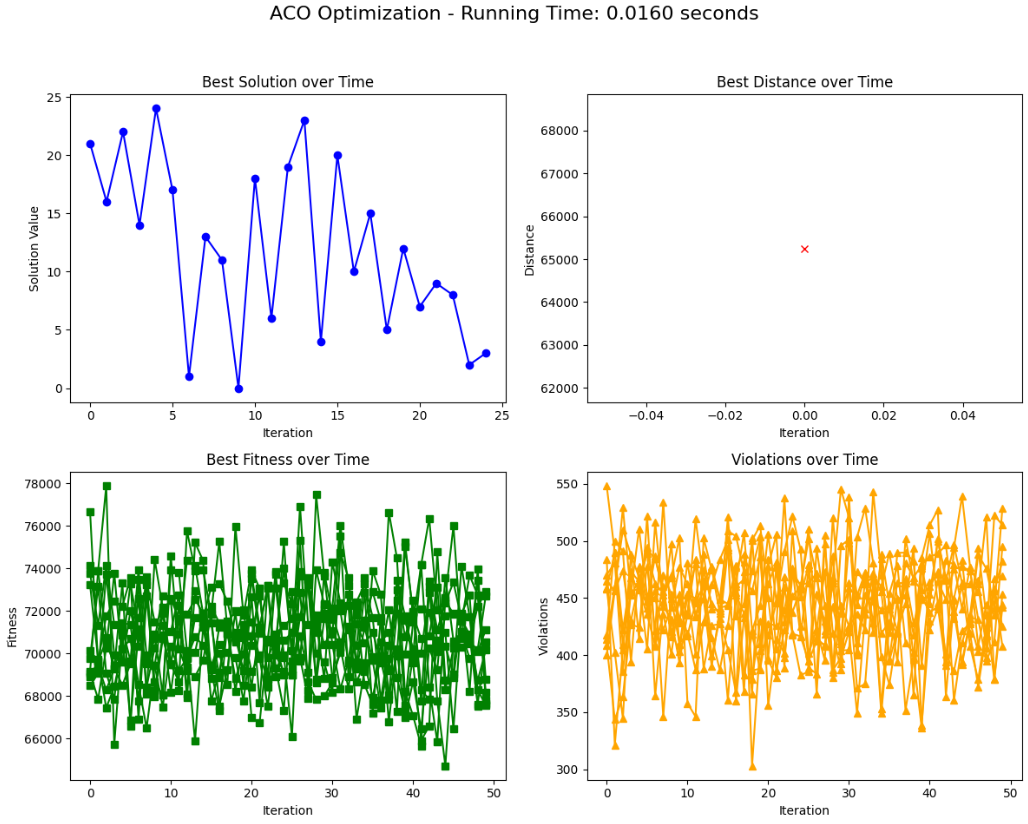
\includegraphics[width=1\linewidth]{figures/Aco_Results.PNG}
    \caption{ACO Algorithm Analysis}
    \label{fig:ACO_Analysis}
\end{figure}

\begin{figure}[H]  % The 'H' forces LaTeX to place the figure here
    \centering
    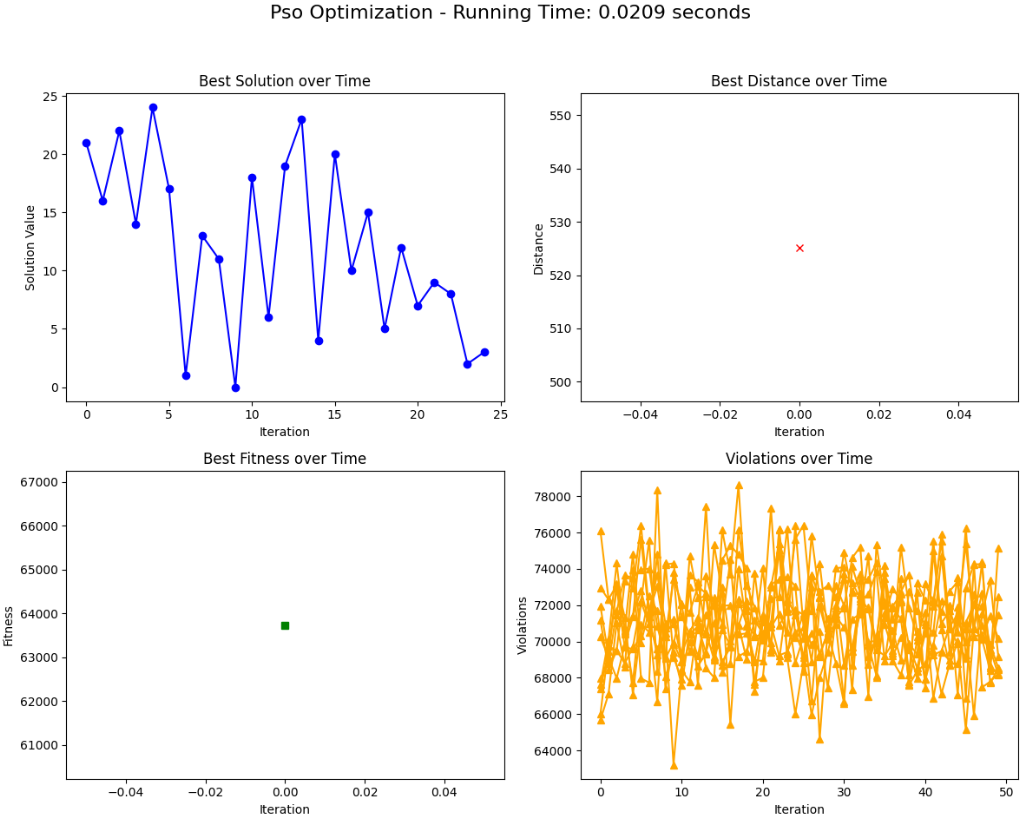
\includegraphics[width=1\linewidth]{figures/Pso_Results.PNG}
    \caption{PSO Algorithm Analysis}
    \label{fig:PSO_Analysis}
\end{figure}

 


